\documentclass[main.tex]{subfiles}

\begin{document}
\sloppy

\section{Post earthquake human presence detection}\label{sec:PostEarthquake}
Durante un terremoto ad elevata magnitudo si possono verificare dei danni a strutture e persone coinvolte. Il progetto SeismoCloud possiede un sistema \emph{Earthquake Early Warning} (EEW), che mira ad avvisare le persone dell'arrivo di un terremoto prima che questo possa raggiungerli, così da ottenere del tempo prezioso per mettersi al sicuro.\newline
\begin{quote}
Fortunatamente per l'umanità, i terremoti più grandi sono allo stesso tempo meno frequenti di quelli piccoli, di circa un fattore 10. [...] Maggior parte l'energia sismica viene rilasciata dai pochi grandi e principali terremoti. La tabella \ref{fig:earthquake-estimation} fornisce una panoramica sulla terminologia utilizzata per caratterizzare la dimensione del terremoto e il tasso medio annuo in tutto il mondo. Il numero di decessi annuali per terremoti, tuttavia, non è necessariamente correlato ai grandi e maggiori terremoti. I terremoti forti e persino moderati che si verificano al di sotto di aree popolate e vulnerabili possono causare danni significativi e maggiori perdite di vite umane rispetto a un grande terremoto di subduzione, ad esempio, nelle Isole Aleutine. L'area di rottura di un terremoto aumenta con la magnitudo, una stima approssimativa può essere calcolato usando l'equazione: \[\log_{10}(Area) = 2/3M-2.28\] Come regola generale: magnitudine M5 il terremoto causa danni in una zona con un diametro intorno ai 3 km, un M6 circa \(20\)km, M7 \(\sim{70}\)km e M8 \(\sim{200}\)km. I più grandi terremoti come l'evento del Cile del 1960 \(M_w=9.4\) hanno causato danni in un diametro fino a 1000 km.\cite{EarthquakePrediction}

\begin{figure}[H]
    \centering
    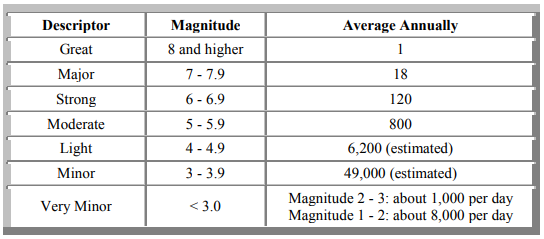
\includegraphics[]{img/Post-Earthquake/earthquake-estimation.PNG}
    \caption{Numero medio di terremoti per intervalli di magnitudo diversi\cite{EarthquakePrediction}.}
    \label{fig:earthquake-estimation}
\end{figure}
\end{quote}
Nell'articolo di S. Wiemer, ci viene quindi mostrata una media globale annuale dei terremoti e le loro intensità. Oltretutto vengono fornite delle importanti stime dell'area interessata all'aumentare della magnitudo. Ciò comporta che più alta sarà la magnitudo, maggiore sarà il livello di distruttività e il numero delle persone colpite.\newline
Un EEW è molto utile per permettere alle persone di mettersi al sicuro in tempo. Tuttavia nel caso vengano danneggiate parzialmente o totalmente le strutture le persone che sono riuscite  a mettersi in salvo potrebbero aver bisogno urgentemente di soccorso. Perciò vi è la necessità di offrire ai soccorritori tutti i dati collezionati da SeismoCloud utili ad individuare tempestivamente possibili superstiti, facendo affidamento anche su un modello di \emph{machine learning} in grado di individuare presenza umana attraverso l'audio del telefono.

\subsection{Analisi del problema}\label{sec:analisi-problema}
Il libro \say{Search \& Rescue Operations in Earthequakes}\cite{searchAndRescue} presenta in modo dettagliato informazioni utili all'analisi e comprensione del problema, così che si possa avere un solido punto di partenza.
% Inizio citazione del libro 
\begin{quote}
Le rovine che risultano da un crollo totale hanno due caratteristiche molto importanti:
\begin{itemize}
    \item L'esistenza di un numero sufficiente di \say{\emph{survival spaces}}
    \item Stabilità del volume delle rovine
\end{itemize}
Queste due caratteristiche sono le principali linee guida per l'autoprotezione e per la metodologia delle operazioni di soccorso.
[...]\newline
Le caratteristiche generali del salvataggio da un edificio che ha
subito il collasso totale sono:
\begin{itemize}
    \item Maggiori possibilità di lesioni gravi e perdita di coscienza delle persone intrappolate
    \item Procedure laboriose e dispendiose per localizzare le vittime
    \item La penetrazione delle rovine e l'avvicinamento delle vittime è a procedura particolarmente ardua, laboriosa e dispendiosa in termini di tempo
    \item Stabilità volumetrica del rudere che non viene disturbata nemmeno da scosse di assestamento. Pertanto il rischio di infortunio della squadra di soccorso è nullo.
\end{itemize}

Caratteristiche di un edificio parzialmente crollato:
\begin{itemize}
    \item Le vie di fuga sono bloccate (scale, corridoi, ascensori, porte ecc.)
\item Il materiale da costruzione potrebbe cadere su di loro
\end{itemize}
Le operazioni di soccorso in questi edifici sono diverse da quelle, condotti in strutture che hanno subito un crollo totale, e hanno importanti vantaggi e svantaggi. I vantaggi sono:
\begin{itemize}
    \item L'approccio alle vittime di solito è molto più veloce senza perdere tempo in penetrazioni
\item La maggior parte dei residenti riescono ad evacuare l'edificio dopo il terremoto oppure non sono gravemente feriti
\end{itemize}

Gli svantaggi sono:
\begin{itemize}
    \item Gli edifici nel loro complesso o parzialmente, hanno subito un importante calo del portamento e sono instabili, qualcosa che si pone come una minaccia importante sia per i soccorritori che per le vittime, in caso di scossa di assestamento
\end{itemize}
\cite{searchAndRescue}
\end{quote}

Come viene evidenziato nel libro i problemi principali, a cui vorremmo ovviare, derivano nel caso del collasso totale di una struttura. Infatti vi è in una situazione di estrema emergenza e le vittime potrebbero essere gravemente ferite o prive di coscienza, inabili di poter segnalare la loro presenza all'esterno. Durante il soccorso vi è una lunga fase di ricerca, in cui bisogna scavare nelle rovine per trovare i superstiti, perciò offrire informazioni come la posizione esatta, la presenza umana rilevata e un feedback (se presente) dall'utente colpito dal terremoto possono aiutare significativamente i soccorsi, rendendo gli scavi maggiormente precisi e mirati. 

\subsection{Human presence detection}
Per eseguire la \say{human presence detection} viene usato un modello chiamato \emph{BNS}, creato da Gianmarco Cavallaccio nella sua tesi magistrale\cite{TesiBNS}, su cui è stato applicato il \emph{transfer learning} con YAMNet, una deep net pre-addestrata che prevede 521 classi di eventi audio basate sul corpus AudioSet-YouTube\cite{YAMNet}, per riconoscere anche il respiro, rumore e silenzio prodotti da una persona.
\begin{figure}[H]
    \centering
    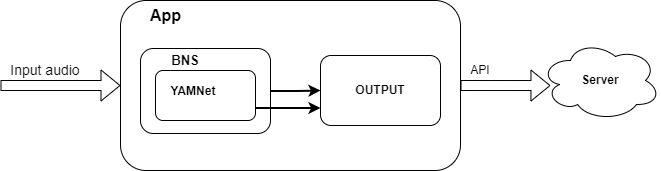
\includegraphics[width=1\linewidth]{img/Post-Earthquake/Post-EQ-Detection-Diagram-BNS chart.png}
    \caption{Diagramma funzionamento app.}
    \label{fig:bns-app}
\end{figure}

\subsubsection{Scalabilità}
BNS verrà incorporato ed eseguito sull'applicazione SeismoCloud, questo permetterà di avere un sistema distribuito in cui ogni telefono eseguirà la detection e comunicherà al server il proprio output. Ciò ottimizzerà le performance e ridurrà notevolmente il traffico di rete, in quanto il server non dovrà eseguire i modelli per \emph{n} telefoni che dovranno inviare numerosi secondi di audio ciascuno.

\subsubsection{BNS output}
Il modello ritorna le classi e la relativa \emph{confidence} di cui verranno prese solo le 3 con attendibilità più alta nel caso di YAMNet più le altre classi aggiunte con BNS. Ad esempio:
\begin{quote}

  {
    modelName: YAMNet,
    detectedType: speech,
    accuracy: 0.8712364
  } \newline
  {
    modelName: YAMNet,
    detectedType: breath,
    accuracy: 0.417391287
  }\newline
  {
    modelName: YAMNet,
    detectedType: singing,
    accuracy: 0.2103823
  }\newline
  {
    modelName: BNS,
    detectedType: speech,
    accuracy: 0.8712364
  }\newline
  {
    modelName: BNS,
    detectedType: silence,
    accuracy: 0.417391287
  }\newline
  {
    modelName: BNS,
    detectedType: speech,
    accuracy: 0.2103823
  }
\end{quote}
\subsection{Design del sistema}
Per sviluppare un buon design per il sistema bisogna comprendere quali devono essere i requisiti fondamentali e come soddisfarli. Il sistema deve offrire un servizio sicuro ed affidabile in grado di ripristinarsi anche nel caso di interruzioni o crash.

\subsubsection{Requisiti}
I requisiti del sistema devono essere:
\begin{itemize}
    \item Efficienza e mantenibilità 
    \item Raccogliere solo i dispositivi coinvolti nel terremoto, così da evitare di raccogliere dati inutili o errati
    \item Mandare una notifica agli utenti coinvolti per chiedere se si trovino in una situazione di pericolo
    \item Raccogliere feedback separando chi sta bene e chi invece potrebbe essere in pericolo
    \item Risvegliare il processo per eseguire la \emph{human presence detection}, se l'utente non ritorna un feedback, mandando una notifica silenziosa al dispositivo
    \item Collezionare i dati raccolti
\end{itemize}
%In questo modo si potranno ottimizzare le chiamate alle API e ridurre il carico di lavoro sul database.\newline
Da questo momento quando si parlerà della notifica che viene inviata all'utente per chiedere se sta bene, ci si riferirà ad essa come \say{\emph{OK notification}}.
\subsubsection{Conclusioni requisiti}
Dai requisiti si comprende che il sistema dovrà consistere di 2 servizi separati ed indipendenti che scambieranno dati tramite il database. Il primo sarà il \say{webapi} che gestirà le API per raccogliere feedback dagli utenti e gli output di BNS, mentre il secondo sarà il \say{worker} che effettuerà la scansione dei terremoti e si occuperà di gestire il sistema di \say{human presence detection}.\newline
Per Notificare gli utenti e attivare il modello di detection ci si affida a \say{Firebase Cloud Messaging} per android e \say{APNS} per iOS. \newline
Per collezionare i dati estenderemo il presente database.

\subsubsection{Cosa sono Firebase e APNS}\label{sec:firebase&apns}
Firebase è una soluzione di messaggistica multi-piattaforma che consente di inviare messaggi in modo affidabile\cite{firebase}, mentre APNS (Apple push notification system) è un servizio di notifica della piattaforma creato da Apple Inc. che consente agli sviluppatori di applicazioni di terze parti di inviare dati alle applicazioni installate sui dispositivi Apple \cite{APNS}.\newline
Firebase e APNS sono i due servizi che verranno usati per mandare notifiche ai dispositivi, rispettivamente, Android e iOS. Ogni client può caricare sul server, tramite API, un token Firebase o APNS; il server usufruendo di questi servizi, potrà usare il token per inviare le notifiche ai rispettivi client.

\subsubsection{Cos'è un evento} \label{sec:evento}
Nella nomenclatura del sistema ci riferiremo al processo che parte dalla rilevazione di un terremoto alla ricerca della presenza umana come \textbf{evento} o \textbf{event}. Nello specifico un \textbf{evento aperto} significa che non è stata ancora attivata la rilevazione della presenza umana. Per \textbf{evento chiuso} si intende che per un dispositivo coinvolto in un terremoto sarà stato effettuato un tentativo di notifica per risvegliare il task della \emph{human presence detection}, oppure questo avrà risposto alla \emph{OK notification}.
\subsubsection{Diagramma design del sistema}
\begin{figure}[H]
    \centering
    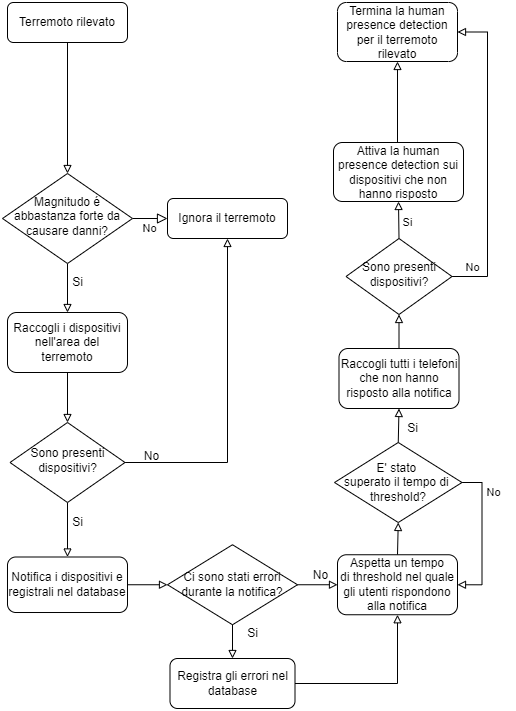
\includegraphics[width=1\linewidth]{img/Post-Earthquake/Post-EQ-Detection-Diagram-flow chart diagram ITA.png}
    \caption{Diagramma del sistema}
    \label{fig:system-diagram}
\end{figure}

\subsection{Progettazione database}
Il database, tenendo conto del diagramma (figura \ref{fig:system-diagram}), deve salvare i seguenti dati:
\begin{itemize}
    \item Telefoni colpiti da un terremoto, con relativi dati
    \item Stato della notifica mandata agli utenti, con relativo errore e risposta
    \item Timestamp dell'invio della notifica, per attivare la detection passato il tempo di threshold
    \item Output del modello BNS
\end{itemize}
Ciò è stato fatto creando due nuove tabelle, una che si occupa di salvare dati relativi alle notifiche e un'altra per l'output del modello.

\subsubsection{OK notification}
La tabella \emph{post\_earthquake\_ok\_notification} serve a salvare le informazioni relative ai dispositivi coinvolti in un terremoto. La tabella è stata progettata in modo da ridurre gli accessi in lettura e scrittura accorpando quante più informazioni possibili.
\begin{figure}[H]
    \centering
    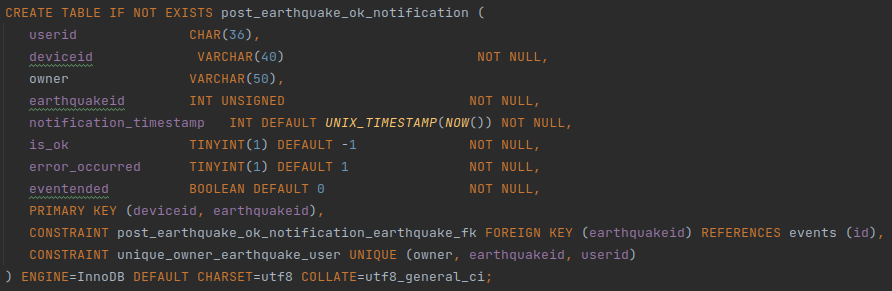
\includegraphics[width=1\linewidth]{img/Post-Earthquake/post-ok-notification-updated.png}
    \caption{Tabella relativa alla \emph{OK notification}}
    \label{fig:ok-not-table}
\end{figure}
Analisi colonne:
\begin{itemize}
    \item userid: identificativo unico per un utente registrato
    \item deviceid: identificativo unico assegnato a un nuovo dispositivo inserito nel database (potrebbe non essere un telefono)
    \item owner: identificativo unico assegnato a un telefono all'installazione dell'applicazione SeismoCloud
    \item earthquakeid: identificativo unico di un terremoto rilevato
    \item notification\_timestamp: Unix timestamp all'inserimento della tupla nella tabella
    \item is\_ok: valore che indica la risposta alla \say{OK notification}, -1 significa che l'utente non ha risposto, 0 che l'utente è in pericolo e 1 l'utente dichiara di stare bene
    \item error\_occurred: indica se si è verificato un errore durante l'invio della \say{OK notification}, di default è 1 in quanto la notifica si suppone non ancora inviata all'inserimento della tupla
    \item eventended: indica se per un utente è stato chiuso l'evento. Un evento, vedi \ref{sec:evento}, viene chiuso in due casi, o quando un utente risponde alla notifica oppure quando viene attivata la detection
\end{itemize}
La chiave primaria sarà data dalla coppia \emph{deviceid} e \emph{earthquakeid}, così ogni tupla sarà identificata dall'id del dispositivo e il terremoto da cui è stato colpito. In questo modo un singolo device potrà essere coinvolto in \emph{n} terremoti, ma non più volte nello stesso.
Una super-chiave sarà quindi la terna \emph{phoneid}, \emph{owner} e \emph{earthquakeid}, per garantire la consistenza delle informazioni. In questo modo non potremo avere tuple duplicate per lo stesso terremoto, ma non escludiamo l'opzione che un utente abbia più dispositivi su cui ha effettuato l'accesso che sono stati coinvolti nello stesso terremoto.\newline
La colonna \emph{eventended} ha il compito di segnare la conclusione di un evento. È stata aggiunta per garantire che gli utenti vengano notificati correttamente, anche in caso di un crash del sistema o di un riavvio. Senza questa colonna, non ci sarebbe modo di sapere se un utente è stato notificato o meno dopo un'interruzione del sistema.

\subsubsection{BNS output}
La tabella \emph{people\_detection\_output} serve a salvare le informazioni relative all'output del modello BNS. Le informazioni vengono inviate dal client al server tramite API.
\begin{figure}[H]
    \centering
    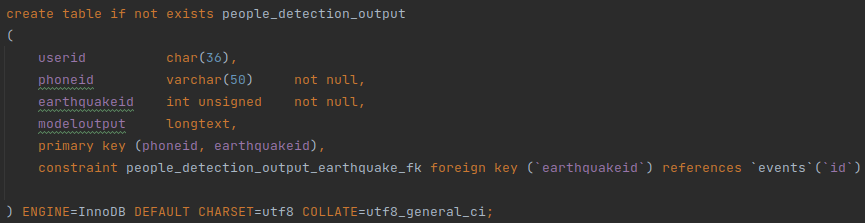
\includegraphics[width=1\linewidth]{img/Post-Earthquake/BNS-output.png}
    \caption{Tabella output BNS}
    \label{fig:BNS-table}
\end{figure}
Analisi colonne:
\begin{itemize}
    \item userid: identificativo unico per un utente registrato
    \item phoneid: identificativo unico assegnato a un telefono all'installazione dell'app\newline SeismoCloud
    \item earthquakeid: identificativo unico di un terremoto rilevato
    \item modeloutput: output del modello BNS in formato JSON
\end{itemize}
La chiave primaria sarà data dalla coppia \emph{phoneid} e \emph{earthquakeid}, in quanto un output è identificato dal telefono di provenienza e il terremoto di origine. \newline
Si è deciso di salvare l'output in formato JSON per ottimizzare gli accessi in lettura e scrittura, piuttosto che creare un'ulteriore tabella.\newline %L'utilizzo del tipo \emph{longtext} per salvare l'output del modello non ha effetto sulle performance in quanto non deve essere indicizzato.
Una soluzione alternativa sarebbe stata di creare un'altra tabella, che chiameremo \emph{BNS\_output} in cui inserire ogni classe rilevata con relativa affidabilità per ogni telefono che avvia la detection. Questa idea è stata scartata per ottimizzare gli accessi in lettura e scrittura nel database.
% oppure duplicare le righe per ogni classe ritornata dal modello. Questo però sarebbe stato un enorme spreco di memoria.


\subsection{API design}
Progettato il database bisogna fare il design delle API con cui comunicheranno i client.\newline
Le API necessarie sono: una per raccogliere le risposte al sondaggio \say{\emph{OK notification}} e un'altra per salvare l'output della \emph{human presence detection}.

\subsubsection{OK-Notification API}\label{sec:OK-notification-API}
L'API per salvare le risposte dell' \say{\emph{OK notification}} è stata sviluppata sotto il seguente percorso \say{/me/earthquake/\{earthquakeid\}/ok-notification}, dove \emph{earthquakeid} indica l'identificatore univoco di un terremoto, quindi la risorsa a cui si fa riferimento.\newline
I parametri dell'API, oltre a quelli di default, saranno:
\begin{itemize}
    \item \emph{earthquakeid}: identificativo unico del terremoto a cui si fa riferimento
    \item \emph{ok-notification-response}: oggetto in formato JSON che contiene le informazioni richieste per la risposta
\end{itemize}
L'oggetto \emph{ok-notification-response} al momento possiede un unico prarametro di tipo booleano \say{isok}. In futuro non si esclude che il numero dei parametri possa crescere, infatti per aumentare la mantenibilità si è preferito incorporare la risposta \say{isok} in una struttura.
\begin{figure}[H]
    \centering
    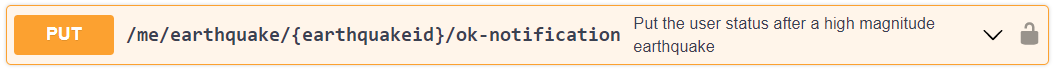
\includegraphics[width=1\linewidth]{img/Post-Earthquake/ok-notification-API-path.PNG}
    \caption{Path ok-notification API}
    \label{fig:OK-notification-path}
\end{figure}
\begin{figure}[H]
    \centering
    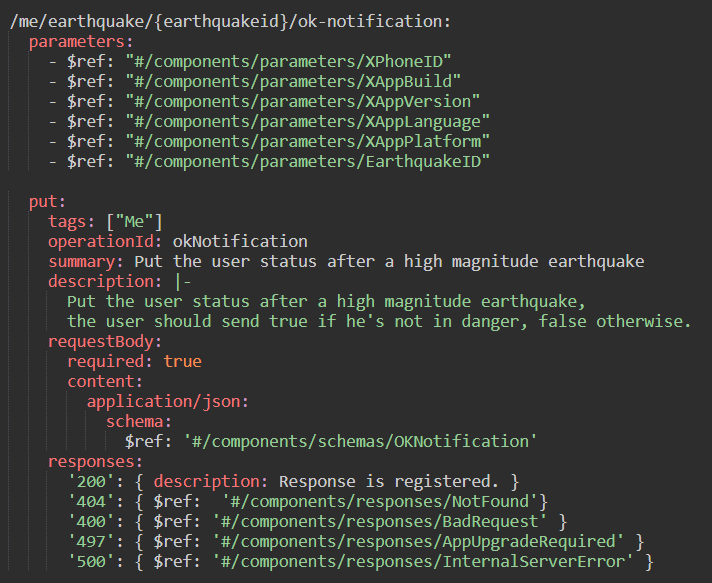
\includegraphics[width=1\linewidth]{img/Post-Earthquake/ok-notification-api.png}
    \caption{Documentazione /me/earthquake/\{earthquakeid\}/ok-notification}
    \label{fig:OK-notification-openapi}
\end{figure}
\begin{figure}[H]
    \centering
    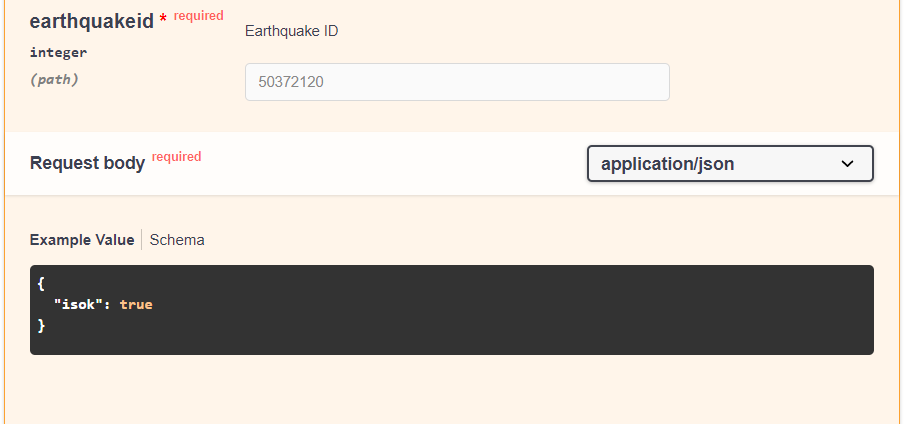
\includegraphics[width=1\linewidth]{img/Post-Earthquake/ok-notification-api-parameters.png}
    \caption{Parametri dell'API /me/earthquake/\{earthquakeid\}/ok-notification}
    \label{fig:OK-notification-openapi-parameters}
\end{figure}


\subsubsection{People-Detection-Output API}
Per salvare l'output di BNS è necessario che il client, dopo aver effettuato la \say{\emph{human presence detection}}, utilizzi l'API \say{/me/earthquake/\{earthquakeid\}/people-detection}, inviando tutti i dati rilevanti raccolti dal modello. Questa dovrà validare l'output del modello ed inserire i dati nel database. L'input di questa API, oltre a quelli di default, sono:
\begin{itemize}
    \item \emph{earthquakeid}: identificativo unico del terremoto a cui si fa riferimento, viene inserito all'interno del path.
    \item \emph{people-detection-output}: array di strutture che contengono il nome del modello, classe rilevata e l'affidabilità dell'output, viene inserito in formato JSON nel body.
\end{itemize}

\begin{figure}[H]
    \centering
    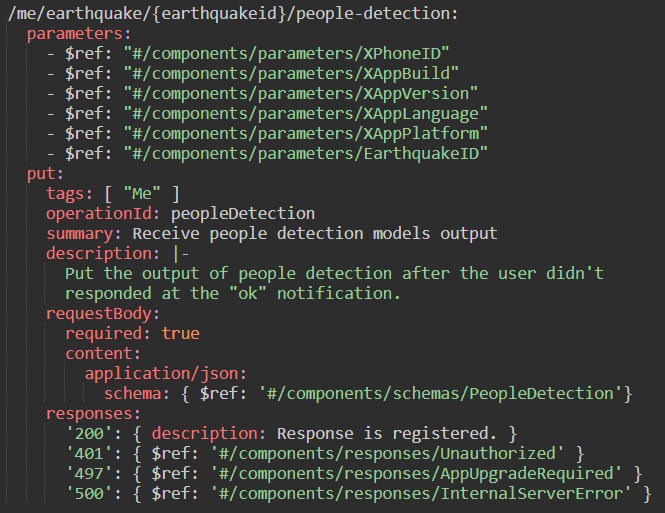
\includegraphics[width=1\linewidth]{img/Post-Earthquake/bns-output-openAPI-doc.PNG}
    \caption{Documentazione /me/earthquake/\{earthquakeid\}/people-detection}
    \label{fig:bns-output-doc}
\end{figure}

\begin{figure}[H]
    \centering
    
\includegraphics[width=1\linewidth]{img/Post-Earthquake/bns-output-API-path.PNG}
    \caption{Path bns-output API}
    \label{fig:bns-output-path}
\end{figure}
\begin{figure}[H]
    \centering
    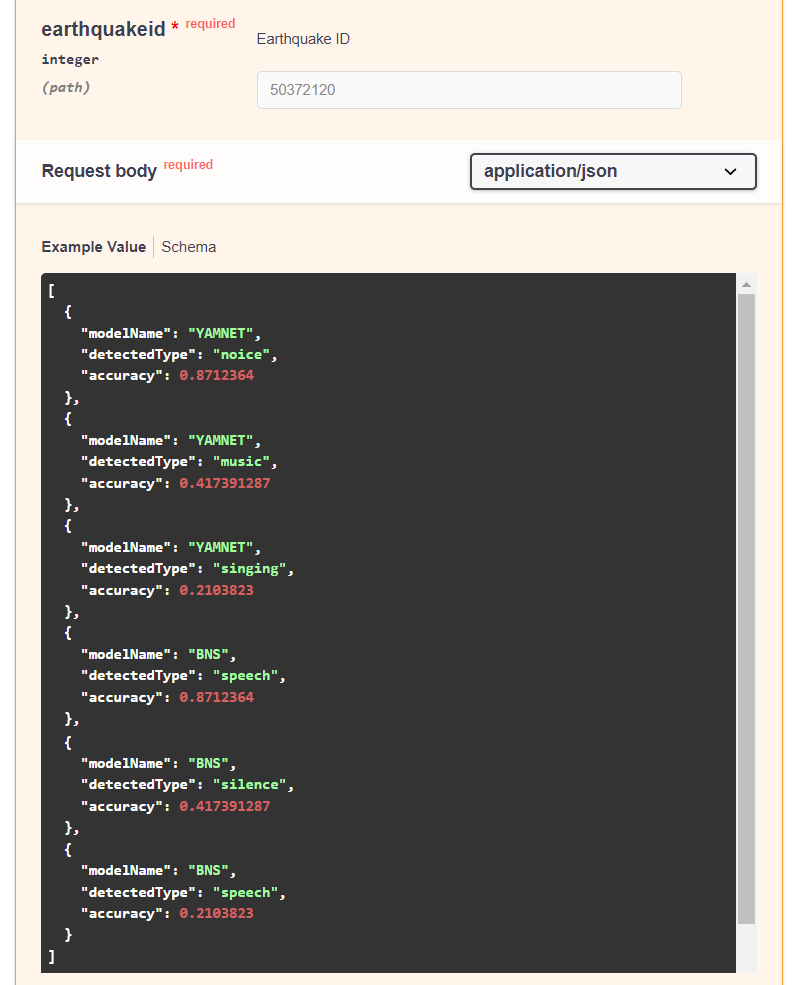
\includegraphics[scale=0.75]{img/Post-Earthquake/bns-output-API-example.PNG}
    \caption{Parametri dell'API /me/earthquake/\{earthquakeid\}/people-detection}
    \label{fig:bns-output-example}
\end{figure}
\newpage
\subsubsection{Implementazione People-Detection-Output API}
Nella seguente funzione andremo ad implementare le operazioni da eseguire alla chiamata dell'API \say{/me/earthquake/\{earthquakeid\}/people-detection}. Quindi, dopo aver controllato la correttezza dei parametri, bisognerà verificare che non siano stati mandati dati inconsistenti dal modello BNS. Per farlo si decodificherà il JSON che contiene gli oggetti di output e ne si verificherà la validità attraverso un metodo apposito. Infine si potrà inserire i dati raccolti nel database.
\lstinputlisting[language=go]{Code/post-eq-people-detection/post-eq-people-detection.go}
A seguire vi è la struttura che modella l'output BNS e il metodo che ne valida il contenuto.
\lstinputlisting[language=go]{Code/post-eq-people-detection/ensure-output-correct-formattation.go}


\subsection{Worker design}\label{sec:workerfdesign}
Dopo aver implementato le API e il database, rimane di progettare il servizio che si occuperà di gestire il sistema (figura \ref{fig:system-diagram}). \newline
Nel progetto \say{SeismoCloud WebAPI} è possibile aggiungere micro-servizi/task asincroni che verranno eseguiti da un processo chiamato \say{worker}. Questi servizi vivono ognuno in una propria \say{goroutine}, ovvero un \say{lightweight thread gestito da Go a tempo di esecuzione}\cite{Goroutine}, generata dal worker.\newline
Per gestire il sistema di \say{post earthquake human presence detection} è necessario aggiungere una nuova task al worker.\newline

\subsubsection{Data pipeline design}
Per ottenere la massima efficienza del sistema è stato progettato un design che prevede la creazione di una \say{data pipeline}, ovvero una serie di processi, ognuno con un compito diverso. In questa pipeline, ogni processo attende e riceve un dato dal precedente, lo elabora, lo passa al successivo e ripete i precedenti passaggi. In questo modo, il dato viene elaborato in modo diverso da ogni processo fino all'ultimo. Ogni processo lavorerà in modo indipendente dagli altri garantendo l'elaborazione di dati parallela.\newline
Il processo relativo all'esecuzione della \emph{data pipeline} per un singolo terremoto può essere visualizzato come un automa a stati finiti (DFA):
\begin{figure}[H]
    \centering
    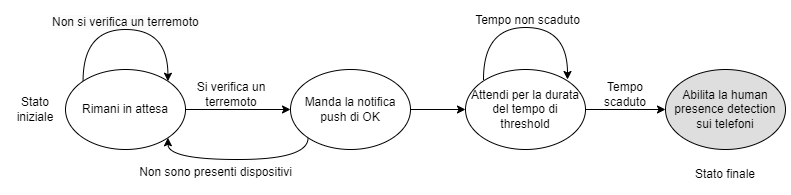
\includegraphics[width=1\linewidth]{img/Post-Earthquake/Post-EQ-Detection-Diagram-Data pipeline automa.png}
    \caption{DFA \emph{data pipeline} relativa a un singolo terremoto}
    \label{fig:Post-EQ-Detection-Diagram-Data pipeline automa}
\end{figure}
Questo automa però presenta un problema: se il sistema dovesse avere un crash o un riavvio mentre il DFA si trova in uno stato non accettante, non vi sarebbe modo di ripristinare il processo e le informazioni saranno inconsistenti.\newline
Per risolvere il problema è stato aggiunto un nuovo stato, all'avvio del processo, che controlla se vi sono \say{eventi aperti} (vedi \ref{sec:evento}).
\begin{figure}[H]
    \centering
    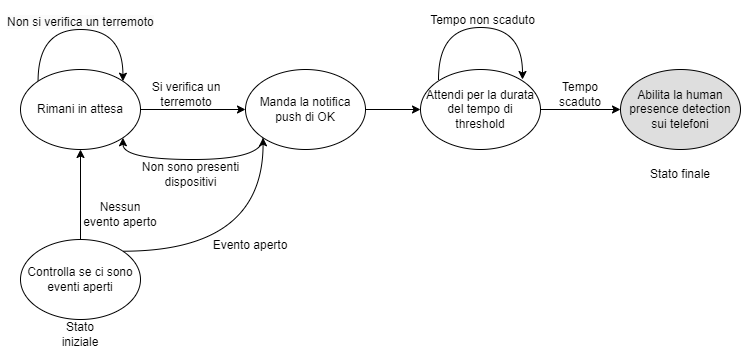
\includegraphics[width=1\linewidth]{img/Post-Earthquake/Post-EQ-Detection-Diagram-Data pipeline automa final.png}
    \caption{DFA \emph{data pipeline} finale relativa a un singolo terremoto}
    \label{fig:Post-EQ-Detection-Diagram-Data pipeline automa final}
\end{figure}


\subsubsection{Event and Event handler}
Per modellare il precedente DFA è stato deciso di usare un sistema ad eventi. Ogni stato dell'automa è descritto da un \say{evento} mentre ogni arco un \say{event handler} che processa l'output dell'evento. Pertanto è stato costruito un gestore di eventi interno al worker.\newline
Per far comunicare gli eventi e gli \emph{event handlers} sono stati utilizzati i \say{\emph{channels}}:
\begin{quote}
Channels are a typed conduit through which you can send and receive values with the channel operator, \(\leftarrow\).
By default, sends and receives block until the other side is ready. This allows goroutines to synchronize without explicit locks or condition variables.\cite{GoChannels}
\end{quote}

Un \say{evento} è un'interfaccia che espone due metodi, uno per l'esecuzione e un' altro per notificare il \emph{listener} (il gestore degli eventi).
\begin{lstlisting}[language=go]
type Event interface {
    Execute(...interface{}) Data
    NotifyListener(data *Data)
}
\end{lstlisting}
Ora serve una struttura che implementi l'evento:
\begin{lstlisting}[language=go]
type eventFunction func([]interface{}) Data // tipo funzione che prende 
// come input un array di quasiasi tipo di dati 
type Data []interface{} // array di quasiasi tipo di dati 

// implementa l'interfaccia Event
type SimpleEvent struct {
    Event      // intefaccia Event
    fn       eventFunction // fuzione da eseguire prima di notificare 
    // l'handler, costituisce le operazioni effettuate dall'evento
    callback eventFunction // funzione che viene chiamata da Execute,
    // necessaria per incapsulare "fn" e "NotifyListener(data *Data)"
    notify   chan Data // canale in cui manda il dato processato 
    // all'handler
    name     string // nome dell'evento
}
\end{lstlisting}
Implementiamo i metodi che verranno esposti fuori dal package:

\begin{lstlisting}[language=go]
func (s *SimpleEvent) NotifyListener(data Data) {
	s.notify <- data  // invia il dato all'handler
}

func (s *SimpleEvent) Execute(i ...interface{}) Data {
	return s.callback(i) // esegue la funzione "fn" e notifica l'handler
}

// crea una nuova struttura SimpleEvent
func NewSimpleEvent(function eventFunction) *SimpleEvent {
    s := SimpleEvent{}
    s.fn = function
    return &s
}

\end{lstlisting}
Un \emph{Handler} invece è un'interfaccia che espone tre metodi:
\begin{lstlisting}[language=go]
type Handler interface {
    Handle(data Data) error // funzione che gestisce un evento
    RegisterEvent(event *SimpleEvent)  // rimane in attesa del 
                                       // verificarsi di un evento
    StartHandler(l logrus.FieldLogger) // avvia la goroutine del
                                       // gestore
}
\end{lstlisting}
Quindi andrà implementata la struttura che incorporerà l'interfaccia
\begin{lstlisting}[language=go]
type handlerFunction func(data Data) error // funzione che gestisce 
                                           // un evento

type SimpleEventHandler struct {
    Handler                 // interfaccia incorporata
    handle handlerFunction  // funzione che gestisce l'evento
    Wait   chan Data        // canale in cui attende per il verificarsi 
                            // dell'evento registrato 
    Kill   chan interface{} // canale in cui aspetta un segnale di 
                            // interruzione
    name   string           // nome del gestore dell'evento
}
\end{lstlisting}
Definiamo una funzione per creare un nuovo \emph{SimpleEventHandler}:
\begin{lstlisting}[language=go]
// crea un nuovo SimpleEventHandler, prende in input una funzione che 
// verra' assegnata all'handler, la funzione esprime le operazioni da 
// effettuare per gestire un determinato evento
func NewSimpleEventHandler(name string, function handlerFunction) 
*SimpleEventHandler {
	var s SimpleEventHandler
	s.Wait = make(chan Data, 1)
	s.Kill = make(chan interface{}, 1)
	s.handle = function // viene assegnata la funzione
	s.name = name
	return &s
}
\end{lstlisting}
Per registrare un evento al suo handler inserisco una nuova funzione nel parametro \emph{callback} del SimpleEvent, andando ad iniettare le funzioni private dell'\emph{event}. In questo modo il \emph{SimpleEventHandler} sarà completamente all'oscuro dell'implementazione delle funzioni dell'\emph{EventHandler}, ma gli sarà garantita la notifica al termine dell'operazione dell'evento.\newline
Grazie a questa implementazione vi è la possibilità di pre-processare i dati prima che questi vengano passati all'handler, senza coinvolgere direttamente l'evento.
\begin{lstlisting}[language=go]
// Questa funzione registra un evento al suo handler.
// Per farlo mette in comunicazione Il SimpleEventHandler e 
// l'EventHandler sullo stesso channel tramite la 
// funzione BindSimpleHandlerAndSimpleEven. Poi viene modificata la 
// funzione callback dell'evento, assegnandogne una nuova 
// che prima chiama "fn" (vedi sopra) e poi notifica il 
// SimpleEventHandler.
func (s *SimpleEventHandler) RegisterEvent(event *SimpleEvent) {
    BindSimpleHandlerAndSimpleEvent(s, event) // set event and event 
            // handler on the same channel

    // inietta la nuova funzione che chiama le funzioni private 
    // del SimpleEvent
    event.callback = func(i []interface{}) Data {
        var data Data = event.fn(i)  
        // pre-processamento dei dati
        event.NotifyListener(data)
        return data
    }
}
\end{lstlisting}
Funzione per gestire un evento, incapsula la funzione passata come input alla creazione:
\begin{lstlisting}[language=go]
func (s *SimpleEventHandler) Handle(data Data) error {
    return s.handle(data) // chiama la funzione che gestisce l'evento.
                   // questa veniva precedentemente passata come input
}
\end{lstlisting}
Questa funzione avvia il loop per un handler:
\begin{lstlisting}[language=go]
func (s *SimpleEventHandler) StartHandler(l logrus.FieldLogger) {
    var killProc interface{} = nil
    var ev Data
    for {
    // permette di rimanere in ascolto su 2 canali contemporaneamente
        select {
        case ev = <-s.Wait: // attendi per la notifica di un evento
        case killProc = <-s.Kill: // attendi il segnale di interruzione
                                  // dal sistema
        }
        if killProc != nil {
            break
        }
        // chiama la funzione per gestire l'evento
        err := s.Handle(ev)
        if err != nil {
            l.Error(err)
        }
        l.Printf("Succeed: %v", ev)
	}
\end{lstlisting}
Una volta definito l'\emph{event handler} per migliorare la mantenibilità bisogna creare una struttura per semplificarne l'aggiunta e rimozione.


\begin{lstlisting}[language=go]
type HandlerMap map[string]*SimpleEventHandler
type HandlerManager struct {
    HandlerMap HandlerMap // tutte le istanze di SimpleEventHandler, 
     // va usato per avviare e fermare tutte le routine 
     // oppure per recuperare le istanze
}
\end{lstlisting}
\begin{lstlisting}[language=go]
// Aggiungi un SimpleEventHandler
func (e *HandlerManager) AddSimpleEventHandler
(value *SimpleEventHandler) bool {
	if _, contains := e.HandlerMap[value.name]; contains {
		return false
	}
	e.HandlerMap[value.name] = value
	return true
}

// Ritorna un EventHandler dal nome
func (e *HandlerManager) GetHandler(handlerName string) 
(*SimpleEventHandler, bool) {
	var h, ok = e.HandlerMap[handlerName]
	return h, ok
}

// Ferma tutti gli EventHandlers che vengono eseguiti
func (e *HandlerManager) KillHandlers() {
	for _, v := range e.HandlerMap {
		v.Kill <- 1
	}
}
\end{lstlisting}
\begin{lstlisting}[language=go]
// tra le costanti andranno messi i nomi degli handler
const (
	SendOkEventHandler = "SendOkEventHandler"
)

// qui andranno creati e aggiunti tutti gli handlers del manager
func InitializeEventHandlerManager() *event.HandlerManager {
	var manager *event.HandlerManager = event.NewEventHandlerManager()
	manager.AddSimpleEventHandler(NewOkSendEventHandler())

	return manager
}

func NewOkSendEventHandler() *event.SimpleEventHandler {
	return event.NewSimpleEventHandler(SendOkEventHandler, 
        HandleSendOkNotification)
}
\end{lstlisting}


\subsection{Analisi del design}
Nonostante la grande efficienza offerta dalla pipeline, questo design rimane estremamente complesso e scarsamente mantenibile. Infatti se si dovessero apportare dei cambiamenti che implicano una modifica dell'automa bisognerà andare a correggere tutti i collegamenti tra gli eventi e i relativi gestori. Inoltre se venissero modificati il tipo di dati che si passano nel corso della pipeline diventerà molto complicato mantenere la corretta comunicazione. Nel caso invece si dovessero verificare degli errori nel corso della pipeline potrebbe risultare estremamente complicato trovarne la causa.\newline
Esempio di comunicazione tra evento e handler: %le implementazioni dell'handler e dell'event non sono realmente importanti:
\begin{lstlisting}[language=go]
// crea l'evento, legalo e registralo all'handler, 
// iniettando la funzione sendOKNotification
sendNotificationEvent := event.NewSimpleEvent(sendOKNotification)
var sendOkEventHandler, ok = 
    w.eventHandlerManager.GetHandler(SendOkEventHandler)
if !ok {
    w.log.Errorf("Event Handler %s not fount in EventHandlerManager", 
    SendOkEventHandler)
}
sendOkEventHandler.RegisterEvent(sendNotificationEvent)

// ...
for _, eq := range earthquakes {
    // ...
    sendNotificationEvent.Execute(eq, w)
}
\end{lstlisting}
Nonostante le prestazioni, come visto in precedenza nell’articolo di S. Wiemer (vedi \ref{sec:analisi-problema}), la distribuzione annuale di terremoti distruttivi non è abbastanza alta da giustificare una tale ottimizzazione. Perciò è stato deciso di cercare un altro approccio al problema.
\subsection{Worker redesign}
Com'è stato appreso nel paragrafo precedente, è preferibile avere un design maggiormente mantenibile sacrificando la massima efficienza.\newline
Il worker è stato riprogettato effettuando \emph{polling} sul database per trovare eventi ancora aperti per cui non è ancora scaduto il tempo di attesa. Quando vengono rilevati dei telefoni dove è scaduto il tempo di attesa, allora verrà attivata la \emph{human presence detection}, nel caso non sia stata registrata una risposta dal client (vedi \ref{sec:OK-notification-API}). \newline

 \subsubsection{Polling}
Il polling sul database è tecnica di programmazione utilizzata per verificare periodicamente se ci sono modifiche. Viene eseguita una query ogni \emph{n} unità di tempo, se vengono rilevate delle modifiche allora si eseguiranno le azioni più appropriate al contesto.\newline
Per ottenere un giusto compromesso tra efficienza e prestazioni, è essenziale trovare la frequenza ideale per raccogliere i telefoni colpiti dal terremoto dal database. Se si utilizzasse una frequenza troppo alta allora si incorrerà in problemi di performance, in quanto si sprecheranno le risorse del server per la maggior parte del tempo. \newline
Se la frequenza sarà troppo bassa, occuperemo il minor quantitativo di risorse ma potrebbe passare troppo tempo dall'invio delle \emph{OK notification} all'attivazione della \emph{human presence detection}. La frequenza ideale trovata è di un minuto, in questo modo si limiterà l'utilizzo delle risorse sul server e il tempo di attesa sarà trascurabile, anche nel caso un terremoto venga rilevato subito dopo l'ultima esecuzione.


\subsection{Implementazione}
In questo paragrafo si esplorerà l'implementazione del sistema.\newline
Per prima cosa va aggiunto il task nelle routine del worker:
\begin{lstlisting}[language=go]
func (w *_worker) ListenAndServe() error {
    //--------------------------------------
    w.log.Info("Worker : Listen And Serve")
    
    // Register here all scheduled tasks
    w.timedTask(1*time.Minute, w.addEvents)
    w.timedTask(1*time.Hour, w.updateStatistics)
    w.timedTask(1*time.Minute, w.updateDevicesExtras)
    
    // viene aggiunto qui il nuovo task inserendo la funzione da
    // eseguire ogni minuto
    w.timedTask(1*time.Minute, w.postEarthquakePeopleDetection)
    
    // Disabled without letting to the linter
    if globaltime.Now().After(time.Date(2030, 1, 1, 1, 1, 1, 1, 
    time.UTC)) {
    w.timedTask(5*time.Second, w.addEventsFromTwitter)
    w.timedTask(1*time.Minute, w.closeChats)
    w.timedTask(2*time.Minute, w.matchChats)
    }
    
    // Wait for shutdown signal
    <-w.shutdownSignal
    w.log.Info("Worker : Stopping scheduled tasks")
    w.shutdown = true
    
    for _, c := range w.wgchan {
    c <- 0
    }
    w.log.Info("Worker : Waiting for tasks")
    w.wg.Wait()
    return nil
}
\end{lstlisting}
La funzione \say{timedTask} prende in input il tempo di attesa prima di rieseguire in loop la \emph{callback}. La \emph{callback} è un metodo senza parametri di input.
\begin{lstlisting}[language=go]
// timedTask calls callback every howoften time.
func (w *_worker) timedTask(howoften time.Duration, callback func()) {
	var shutdown = make(chan interface{}, 1)
	w.wg.Add(1)
	go func() {
		var t = time.NewTicker(howoften)
		for !w.shutdown {
			callback()
			select {
			case <-t.C:
			case <-shutdown:
			}
		}
		w.wg.Done()
	}()
	w.wgchan = append(w.wgchan, shutdown)
}
\end{lstlisting}


\subsubsection{OK notification}
Nel momento in cui viene rilevato un terremoto viene chiamata una funzione per mandare le \emph{OK notifications}. Questa funzione deve prendere i telefoni che rientrano nell'area di effetto del terremoto, controllare che abbiano un token firebase o APNS registrato e mandare le notifiche.


\subsubsection{Inserimento telefoni colpiti dal terremoto nel database}
Per prendere ed inserire i telefoni colpiti, bisogna prima calcolare l'area di percettibilità del terremoto, per farlo si userà il seguente algoritmo:
\lstinputlisting[language=go]{Code/post-eq-people-detection/percectibleupto.go}
Così con l'area di percettibilità e l'origine possiamo calcolare il bounding box del terremoto. Il bounding box contiene il punto in alto a destra e in basso a sinistra delle coordinate di un quadrato circoscritto all'area del terremoto, in modo da delinearlo con solo 2 punti (figura \ref{fig:bbox}).
\lstinputlisting[language=go]{Code/post-eq-people-detection/bbox.go}
\begin{figure}[H]
    \centering
    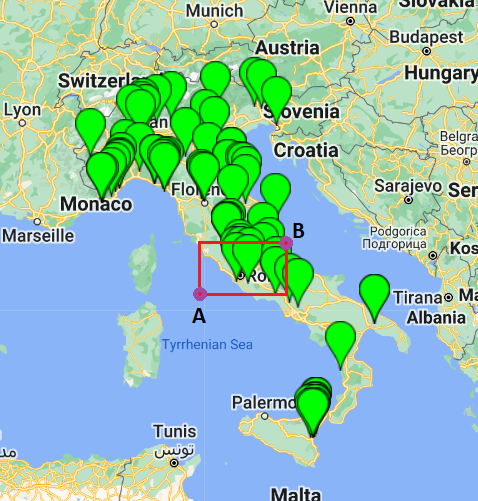
\includegraphics[]{img/Post-Earthquake/bounding-box.PNG}
    \caption{Esempio di bounding box generato dai punti \emph{A} e \emph{B} sulla mappa dei dispositivi}
    \label{fig:bbox}
\end{figure}
Una volta ottenuto il bounding box possiamo sfruttarlo per raccogliere tutti i telefoni che si trovano all'interno della sua area. La seguente query inserisce nella tabella \say{post\_earthquake\_ok\_notification} tutte le tuple che si trovano all'interno del bounding box:
\begin{lstlisting}[language=SQL]
INSERT INTO post_earthquake_ok_notification (userid, deviceid, 
    earthquakeid, eventended, owner)
SELECT DISTINCT d.userid, d.deviceid, ?, 
    IF(EXISTS(
        SELECT pt.phoneid FROM phones_tokens as pt 
        WHERE pt.phoneid = d.owner
        ), 0, 1), d.owner 
-- inserisce 0 per comunicare che l'evento NON e' chiuso
-- inserisce 1 per comunicare che l'evento e' chiuso
FROM devices d
WHERE d.latitude >= ?/*low_lat*/ AND d.latitude <= ?/*max_lat*/
  AND d.longitude >= ?/*low_long*/ AND d.longitude <= ?/*max_long*/;
\end{lstlisting}
Bisogna da notare come l'evento (vedi \ref{sec:evento}) venga chiuso a priori solo per i dispositivi che non sono dotati di un token firebase o APNS in quanto non potranno essere notificati per attivare la \emph{human presence detection}. Ciò viene effettuato durante l'inserimento attraverso la funzione \emph{IF} di MySQL, passando come condizione l'esistenza di un risultato di una query.
\[IF(condition, value\_if\_true, value\_if\_false)\]
In questo modo minimizzeremo il numero di comunicazioni TCP con il database.
I punti interrogativi fungono da placeholder per i valori del bounding box.\newline
La precedente query verrà incapsulata nella seguente funzione:
\lstinputlisting[language=go]{Code/post-eq-people-detection/add-users-phones-to-watching-list.go}


\subsubsection{Raccolta telefoni colpiti dal terremoto}
Per la raccolta dei dati necessari alla notificazione, bisognerà sfruttare, in parte, la query precedente e utilizzare la clausola \emph{INNER JOIN} per unire le informazioni da altre tabelle. 
\begin{quote}
    INNER JOIN: Returns records that have matching values in both tables
\cite{LeftJoin}.
\end{quote}
L'inner join è la scelta migliore in quanto i dispositivi che interessano in questo momento sono solo quelli che possiedono un token \say{firebase} o \say{APNS}, per essere notificati.\newline
Nella seguente query viene utilizzata la funzione \[IFNULL(valore, valore\_alternativo\_se\_NULL)\] 
Restituisce il valore specificato se l'espressione è \emph{NULL}, altrimenti restituisce l'espressione.
Questo controllo è necessario per evitare possibili dati inconsistenti.
\begin{lstlisting}[language=SQL]
SELECT DISTINCT IFNULL(deviceid, ''), IFNULL(pt.type, ''), 
IFNULL(pt.token, '')
FROM devices INNER JOIN phones_tokens pt ON devices.owner = pt.phoneid
WHERE d.latitude >= ?/*low_lat*/ AND d.latitude <= ?/*max_lat*/
  AND d.longitude >= ?/*low_long*/ AND d.longitude <= ?/*max_long*/;
\end{lstlisting}
Le informazioni raccolte sono:
\begin{itemize}
    \item deviceid: identificativo unico di un dispositivo, necessario per aggiornare lo stato di errore dopo la notifica.
    \item type: tipo del token di notifica \say{firebase} o \say{APNS}.
    \item token: codice per notificare il dispositivo.
\end{itemize}
Implementazione della funzione:
\begin{lstlisting}[language=go]
// struttura contenente tutti i dati utili
type UserSendNotification struct {
	Phoneid           string // identificativo del telefono generato 
                            // all'installazione
	NotificationToken string // token per mandare le notifiche
	TypeToken         string // "firebase" o "APNS"
}

func (db *appdbimpl) GetPhonesInEarthquakeBoundingBox(
        box locationutils.BoundingBox) ([]UserSendNotification, error) {
	var userSendNotifications = make([]UserSendNotification, 0)

	err := db.c.Select(&userSendNotifications, `
		select distinct 
    ifnull(deviceid, ''), ifnull(pt.type, ''), ifnull(pt.token, '')
		from devices left join phones_tokens pt on owner = pt.phoneid
		where latitude >= ?/*low_lat*/ and latitude <= ?/*max_lat*/
		and longitude >= ?/*low_long*/ and longitude <= ?/*max_long*/;
	`, box.A.Latitude, box.B.Latitude, box.A.Longitude, box.B.Longitude)

	return userSendNotifications, err
}
\end{lstlisting}
%\subsection{DELETE ME - PROSEGUIRE LA REVISIONE DA QUI}

\subsubsection{Implementazione \emph{OK notification}}
Rilevato un terremoto ad alta magnitudo bisogna richiedere agli utenti un feedback sul loro stato, mandando l'\emph{OK notification}, verificando se l'utente si trovi in uno stato di pericolo; per farlo dovremo raccogliere i token \say{firebase} e \say{APNS} (vedi \ref{sec:firebase&apns}) dal database, per tutti i telefoni che si trovano nel bounding box del terremoto, caricare il payload con informazioni utili ed infine mandare la notifica.\newline
A seguire vi è la funzione esegue i precedenti passaggi, all'interno vi saranno commenti che spiegheranno il processo in modo più dettagliato:
\lstinputlisting[language=go]{Code/post-eq-people-detection/send-ok-notfication.go}

\subsubsection{Implementazione raccolta informazioni per eventi attivi}
Prima di proseguire nell'implementazione dell'attivazione della \say{\emph{post earthquake human presence detection}} bisogna osservare i dati raccolti dal database. Con la seguente query si raccolgono:
\begin{itemize}
    \item deviceid: identificativo di un telefono colpito
    \item earthquakeid: identificativo del terremoto
    \item notification\_timestamp: data e orario formato UNIX in cui è stata effettuato il tentativo per l'\emph{OK notification}
    \item type: tipo del token di notifica \say{firebase} o \say{APNS} 
    \item token: codice per mandare le notifiche ai client
\end{itemize}
I dispositivi da raccogliere vengono scelti attraverso alcuni parametri: l'evento del dispositivo deve essere aperto, quindi non ha risposto alla \emph{OK notification} (\(is\_ok < 0\)), e non è ancora stata effettuato il rilevamento tramite audio.  
\begin{lstlisting}[language=go]
func (db *appdbimpl) GetPostEarthquakeOkNotificationActiveEventResults() 
([]dbtypes.PostEarthquakeOkNotificationResult, error) {
    var results = make([]dbtypes.PostEarthquakeOkNotificationResult, 0)
    err := db.c.Select(&results, `
        SELECT DISTINCT post_earthquake_ok_notification.deviceid,
        earthquakeid,notification_timestamp, phones_tokens.type, 
        phones_tokens.token
        FROM post_earthquake_ok_notification INNER JOIN phones_tokens
        ON post_earthquake_ok_notification.owner = phones_tokens.phoneid
        WHERE eventended = 0 AND is_ok < 0;
        `)
    
    if err != nil {
        return nil, err
    }
    
    return results, nil
}
\end{lstlisting}
\begin{lstlisting}[language=go]
type PostEarthquakeOkNotificationResult struct {
	Deviceid              string `db:"deviceid"`
	Earthquakeid          int64  `db:"earthquakeid"`
	NotificationTimestamp int64  `db:"notification_timestamp"`
	IsOk                  int8   `db:"is_ok"`
	NotificationToken     string `db:"token"`
	NotificationType      string `db:"type"`
}
\end{lstlisting}
\subsubsection{Implementazione chiusura eventi attivi}
Una volta che è stata attivata la rilevazione audio su un client, non essendo più necessario notificarlo nuovamente, bisogna chiudere l'evento aperto associato al terremoto. Per farlo si passeranno tutti gli utenti per cui si vuole chiudere l'evento e l'identificativo del terremoto associato.
\begin{lstlisting}[language=go]
func (db *appdbimpl) ClosePostEarthquakeForNotifiedUsers(earthquakeid 
        int64, phoneids []string) error {
    // prepara la query e i suoi dati
    query, args, err := sqlx.In(`
        UPDATE post_earthquake_ok_notification 
        SET eventended = 1 
        WHERE earthquakeid = ? AND deviceid IN(?);`
        , earthquakeid, phoneids)
    if err != nil {
        return err
    }
    // esegui la query
    _, err = db.c.Exec(query, args...)
    return err
}

\end{lstlisting}

\subsubsection{Implementazione attivazione \emph{post earthquake human presence detection}}
Una volta osservato il sistema, viste le API e le implementazioni delle query che usa il worker, si può proseguire alla realizzazione.\newline
All'interno del \emph{worker} ogni minuto andranno eseguiti i seguenti task:
\begin{itemize}
    \item Raccogli i dispositivi che hanno attivo un evento
    \item Passato il tempo di \emph{threshold} notifica il dispositivo, attivando la detection
\end{itemize}

Dopo aver mandato l'\emph{OK notification} bisognerà risvegliare il processo per la \say{\emph{human detection}} sul dispositivo del client. Quindi bisognerà aspettare un tempo di \emph{threshold} per dare il tempo all'utente di rispondere:
\begin{lstlisting}[language=go]
// costante, tempo da aspettare dopo aver mandato l' "OK notification"
// all'utente
const (
    SendStartDetectionNotificationWaitingTime = 15 // minutes
)
\end{lstlisting}
Prima di proseguire nell'implementazione, è stata dichiarata la seguente struttura, questa serve a incapsulare la lista dei dispositivi che devono essere notificati insieme agli identificativi dei dispositivi associati. In questo modo si potrà notificare e successivamente chiudere l'evento per i dispositivi. 
\begin{lstlisting}[language=go]
type wrapTokens struct {
    sendNotificationDetectionListFirebase []string // list firebase 
                                 // tokens for sending notification
    sendNotificationDetectionListApns     []string // list apns tokens 
                                 // for sending notification
    phoneids                              []string // will be used for 
                                 // closing the event in the database
}
\end{lstlisting}
A seguire vi è il metodo del worker che invia la notifica:
\begin{lstlisting}[language=go]
func (w *_worker) postEarthquakePeopleDetection() {
    results, err :=      
        w.scsdb.GetPostEarthquakeOkNotificationActiveEventResults()
    if err != nil {
        w.log.WithError(err).Error("post earthquake human presence 
                    detection, can't get active events")
        return
    }
    // se non ci sono dispositivi coinvolti in un terremoto non 
    // vi e' bisogno di andare avanti per questa iterazione
    if len(results) == 0 {
        w.log.Debug("post earthquake human presence detection, 
                    no results")
        return
    }

    // crea una mappa che ha come chiave il terremoto di riferimento e
    // come valore la struttura "wrapTokens". Viene utilizzata una mappa 
    // in modo da poter gestire efficacemente anche multipli terremoti 
    // nello stesso istante.
    var earthquakeTokenMap = getEarthquakeTokensMap(results)
    for k, v := range earthquakeTokenMap {
        // manda le notifiche agli utenti coinvolti nel terremoto,
        // ovvero la chiave
        _, err := sendStartDetectionNotification(k, 
                  v.sendNotificationDetectionListFirebase, 
                  v.sendNotificationDetectionListApns, 
                  w)
        if err != nil {
            w.log.WithError(err).Errorf("can't send 'start detection 
                    notification' for earthquake %v", k)
        }
    }
    
    for k, v := range earthquakeTokenMap {
        // chiude gli eventi per i dispositivi notificati
        err = w.scsdb.ClosePostEarthquakeForNotifiedUsers(k, v.phoneids)
        if err != nil {
            w.log.WithError(err).Errorf("can't close post earthquake 
                human presence detection event for earthquake '%v'", k)
        }
    }
}
\end{lstlisting}
La funzione \say{getEarthquakeTokensMap}, come spiegato in precedenza, associa all'identificativo di un terremoto una lista di token \say{firebase} e \say{APNS} ed una lista di ID dei telefoni associati. Queste informazioni vengono incapsulate nella struttura \say{wrapTokens}.
\begin{lstlisting}[language=go]
func getEarthquakeTokensMap(postEarthquakeNotificationResult 
[]dbtypes.PostEarthquakeOkNotificationResult) map[int64]*wrapTokens {
    eqidTokens := make(map[int64]*wrapTokens) // crea la mappa

    // itera sui terremoti
    for _, earthquake := range postEarthquakeNotificationResult {
        // controlla se il tempo di threshold sia passato
        if  !isElapsedWaitingTime(
                time.Unix(earthquake.NotificationTimestamp, 0)
            ) {
            // se non e' passato il tempo ignora il dispositivo
            continue
        }
        
        eqid, exists := eqidTokens[earthquake.Earthquakeid]
        // verifica se esistela chiave nella mappa
        if !exists {
            // se non esiste crealo e inserisci una nuova struttura 
            // associata al terremoto
            eqid = &wrapTokens{
                sendNotificationDetectionListFirebase:make([]string, 0),
                sendNotificationDetectionListApns:    make([]string, 0),
                phoneids:                             make([]string, 0),

            }
            eqidTokens[earthquake.Earthquakeid] = eqid
        }
        // inserisci il token nella lista corretta
        if earthquake.NotificationType == "firebase" {
            eqid.sendNotificationDetectionListFirebase = 
                append(eqid.sendNotificationDetectionListFirebase, 
                       earthquake.NotificationToken)
        } else if earthquake.NotificationType == "apns" {
            eqid.sendNotificationDetectionListApns = 
                append(eqid.sendNotificationDetectionListApns,     
                       earthquake.NotificationToken)
        }
        
        // aggiungi l'identificativo dei device nella lista
        eqid.phoneids = append(eqid.phoneids, earthquake.Deviceid)
    }
    return eqidTokens
}
\end{lstlisting}
\begin{lstlisting}[language=go]
// controlla se sono passati 15 
// minuti dal timestamp della "OK notification"
func isElapsedWaitingTime(startTime time.Time) bool {
  elapsed := time.Since(startTime)
  return elapsed.Minutes() >= SendStartDetectionNotificationWaitingTime
}
\end{lstlisting}
La funzione \say{sendStartDetectionNotification} invia le notifiche ai token  \say{firebase} e \say{APNS} passati in input. La notifica è silente, in quanto non genera suono e non contiene ne il titolo ne una descrizione, bensì solo un \emph{payload} con informazioni utili da offrire al client per comunicare con le API:
\begin{lstlisting}[language=go]
func sendStartDetectionNotification(earthquakeid int64, w *_worker,
        firebaseTokens []string, apnsToken []string) 
        (mobilepush.PushResult, error) {
    customDataMap := make(map[string]string)
    customDataMap["x-sc-category"] = "start-detection"
    customDataMap["x-sc-earthquakeid"] = strconv.FormatInt(
        earthquakeid, 10)
    
    var detectionNotification = mobilepush.Notification{
        CustomData:     customDataMap,
        FirebaseTokens: firebaseTokens,
        ApnsTokens:     apnsToken,
        Title:          fmt.Sprintf("Start human presence detection for 
            earthquake %v", earthquakeid),
    }
    return w.push.SendPush(detectionNotification)
}
\end{lstlisting}
\end{document}